\documentclass[12pt,hyperref,a4paper,UTF8]{ctexart}
\usepackage{BNUpapers}
\usepackage{listings}
\usepackage{xcolor}

% 可选：设置代码样式
\lstset{
    language=Python,
    basicstyle=\ttfamily\footnotesize,
    keywordstyle=\bfseries\color{blue!70!black},
    commentstyle=\itshape\color{gray!50!black},
    stringstyle=\color{orange},
    breaklines=true,
    backgroundcolor=\color{gray!5},
    frame=none,
    numbers=left,
    numberstyle=\tiny\color{gray!60},
    numbersep=5pt,
    tabsize=4
}
%%-------------------------------正文开始---------------------------%%
\begin{document}

%%-----------------------封面--------------------%%
\cover

%%------------------摘要-------------%%
%\begin{abstract}
%
%在此填写摘要内容
%
%\end{abstract}

\thispagestyle{empty} % 首页不显示页码

%%--------------------------目录页------------------------%%
\newpage
\tableofcontents

%%------------------------正文页从这里开始-------------------%
\newpage

\section{研究背景与任务意义}

\subsection{智慧课堂与教育数字化}

随着信息技术的快速发展，教育数字化已成为全球教育改革的核心趋势。在国内，2025年《教育强国建设规划纲要(2024-2035年)》明确提出实施国家教育数字化战略，促进人工智能助力教育变革。2025年4月，教育部等九部门印发《关于加快推进教育数字化的意见》，提出以“人工智能+教育”为抓手，推动人工智能融入教育全要素、全过程、全场景。目前，国家智慧教育平台已成为世界规模最大的高质量数字教育平台，为数字化教学资源共建共享奠定了坚实基础。

在国际上，美国国家教育技术计划(NETP)持续推进数字化教育转型，欧盟推出European Digital Education Action Plan强调AI赋能教学评估，联合国教科文组织发布面向学生和教师的全新人工智能能力框架，指导各国支持师生了解人工智能的潜力与风险，以便在教育领域及其他领域以安全、合乎伦理且负责任的方式运用人工智能。这些政策举措共同表明，利用人工智能技术提升教学质量和学习效果已成为国际教育发展的重要方向。

智慧教室作为教育数字化的重要载体，正在国内高校规模部署。智慧教室系统集成高清录播、智能物联、巡课督导、无感考勤等功能，实现了课堂教学过程的全程记录与智能分析。AI教学分析课堂质量评估系统在多所高校试点应用，与专家评分的一致性达到91.3\%，评估效率提升20倍以上，显示出人工智能技术在课堂教学评估中的巨大潜力。

\subsection{学生课堂参与度与注意力分析}

学生课堂参与度(Student Engagement)是衡量学习质量和教学效果的核心指标。从教育学理论出发，学生参与度可划分为三个维度：行为参与度(Behavioral Engagement)涉及学生的肢体动作、课堂出勤和任务完成情况；情感参与度(Affective Engagement)涵盖学生的情感状态、学习兴趣和内在动机；认知参与度(Cognitive Engagement)则关注学生的深度学习策略和知识建构过程。

在课堂场景中，头部姿态(Head Pose)被认为是评估学生行为参与度的有效代理指标。大量研究表明，学生的抬头率(looking-up rate)与他们对教学内容的注意力高度相关——当学生抬头注视教师或课件时，通常表明他们正在接收和加工教学内容；而低头行为可能表示学生正在做笔记、独立思考或出现注意力分散。因此，通过计算机视觉技术检测学生的抬头/低头状态，计算课堂抬头率，可以有效评估学生的课堂参与程度。

然而，需要指出的是，低头行为并不总是等同于注意力分散。学生在课堂中可能因以下正当原因低头：记录课堂笔记、独立思考和内化知识、阅读课本或学习材料、开展课堂练习等。这意味着，单纯的低头率统计可能无法准确反映真实的课堂参与情况，需要结合教学内容特征进行综合分析。

\subsection{自动化课堂分析的必要性}

传统的课堂质量评估主要依赖人工听课或课后问卷调查，这种方式存在明显局限：其一，样本量小且主观性强，不同评估者对同一课堂的评价可能存在显著差异，难以保证评估的客观性和一致性；其二，无法捕捉课堂动态变化过程，课堂教学是一个时变的复杂过程，静态的听课记录难以反映教学效果的完整变化轨迹；其三，时效性差，反馈滞后，传统的听课评课往往在课后进行，无法为教师提供实时的教学调整依据。

基于计算机视觉的自动化课堂分析系统可以有效解决上述问题。该系统能够实现无感采集，在不干扰正常教学秩序的前提下获取课堂数据，保护学生隐私和正常的课堂生态；能够实现全时段、多维度的数据采集，覆盖整堂课而非单个时间切片，捕捉完整的教学过程；能够提供实时反馈，支持教师及时调整教学策略，实现精准教学干预。

此外，随着课堂录播系统的普及，高校积累了大量课堂教学视频资源。这些视频中蕴含着丰富的教学行为数据和学生的学习行为信息，但目前大多未被有效挖掘和利用。开发自动化课堂分析系统，可以充分利用这些沉睡的数据资产，为教学研究和教学改进提供数据支撑。

\subsection{本项目的任务与意义}

本项目构建了基于“双摄像机协同分析”的课堂视频分析系统，通过同时采集课件视频与学生视频，从“教学内容”和“学生课堂状态”两个角度对课堂过程进行联合分析。系统实现了课件内容识别、学生抬头率统计以及时间轴融合分析等功能。项目的研究意义体现在以下几个方面：

\begin{itemize}
    \item 引入双摄像机协同方案，分别针对课件识别与学生行为分析进行优化，相较于单摄像机方案能够有效降低遮挡、视角偏移等问题对识别效果的影响，提高系统的实用性。

    \item 项目关注“教学内容”与“学生注意力”之间的相关性分析，不仅停留在单模态的课件识别或行为检测层面，而且建立了教学内容特征与学生课堂反应之间的关联关系，为课堂教学质量评估提供了量化依据。

    \item 项目充分考虑课堂场景的特殊性，如课件透视畸变、学生密集遮挡、光照变化等实际挑战，设计并实现了相应解决方案，提高了系统在真实课堂环境中的鲁棒性。
\end{itemize}

\section{问题定义与任务拆解}

\subsection{系统任务框架}

本项目构建双摄像机协同分析系统，对课堂视频中的课件内容与学生行为进行联合分析。系统由两条分析链路组成：

摄像机1（后置）分析链路：后向前拍摄方式，采集教师授课区域与PPT课件内容，输出课件文本内容和页面停留时间。

摄像机2（前置）分析链路：前向后拍摄方式，采集学生区域与课堂行为，输出学生人数和实时抬头率。

最终，系统基于时间戳对两条链路的结果进行对齐融合，输出每页PPT对应的平均抬头率、整堂课平均抬头率以及抬头率变化趋势，结合课件切换情况对课堂效率进行综合分析。

\subsection{子任务一：课件内容检测与识别}

课件内容检测与识别是从课堂视频中提取PPT文本信息的关键步骤，其技术流程包括课件区域提取、透视矫正、文字检测与识别、课件切换检测和页面停留时间统计。
% 在课件区域提取环节，由于课堂摄像机可能存在水平偏移、俯仰角变化，课件区域在图像中通常表现为四边形区域而非标准矩形。本项目采用传统图像处理方法进行课件区域提取，包括灰度化、去噪、边缘检测、轮廓提取、多边形拟合和透视变换等步骤，获得整齐的课件画面。

% 文字检测与识别环节采用OCR技术完成课件内容提取。在文本检测方面，可采用传统阈值分割方法或DBNet等深度学习方法检测文本区域；在文字识别方面，可采用CRNN或PaddleOCR等方法进行序列识别。通过OCR识别结果可以获得当前PPT页面的文本内容。

% 课件切换检测通过比较相邻时间段OCR识别结果之间的差异实现。若文本内容变化较小，则认为课件页面未切换；若文本内容变化明显，则认为课件页面发生切换。通过记录页面切换时刻建立完整的PPT页面时间轴。

% 本子任务的主要技术挑战包括：透视畸变导致的文字变形、模糊或低分辨率视频导致的识别困难、公式和特殊符号的混淆等。

\subsection{子任务二：学生抬头检测与注意力分析}

学生抬头检测与注意力分析是评估学生课堂参与情况的核心环节，技术流程包括学生人数统计、人脸检测、抬头状态判定和抬头率计算。
该子任务面向前置摄像机画面，对学生座位区域进行抽帧分析。系统采用头部状态检测模型识别可见学生头部，并将目标划分为抬头和低头两类，再根据有效检测目标数量计算当前帧抬头率。与只统计人脸可见数量的方法相比，该流程能够在部分侧脸、远距离和低头状态下保留更多头部姿态信息。
% 学生人数统计采用YOLO系列目标检测算法对课堂视频中的学生目标进行检测。训练数据来源包括GitHub开源项目、公开数据集（Kaggle、Roboflow等）以及自行采集标注的课堂视频。课堂环境中的特殊挑战包括学生遮挡、光照变化、学生坐姿差异和远距离小目标等。

% 人脸检测同样采用YOLO人脸检测模型定位学生人脸区域。在获得人脸检测结果后，通过以下规则判断学生是否处于抬头状态：检测到完整人脸时认为学生处于抬头状态，未检测到人脸或仅检测到头顶部区域时认为学生处于低头状态。后续可进一步结合头部姿态估计与面部关键点检测提高准确率。

% 抬头率计算公式为 $R = \frac{M}{N} \times 100\%$，其中 $N$ 为学生总人数，$M$ 为检测到人脸的学生人数。进一步地，可基于时间戳统计每页PPT对应时间段内的平均抬头率。

% 本子任务的主要技术挑战包括：小目标检测（远距离学生人脸可能小于30像素）、密集人群遮挡、快速头部姿态变化、长时间追踪中的ID切换等。

\subsection{子任务三：教学内容与注意力相关性分析}

教学内容与注意力相关性分析是建立“课件内容”与“学生课堂行为”之间对应关系的关键步骤，也是实现课堂效率评估的核心。
% 时间轴对齐是两路视频结果融合的前提。由于课件识别流程与学生行为分析流程分别来自两路视频，需要基于时间戳对两路结果进行对齐：将每一页PPT的停留时间区间与对应时间段内的抬头率数据进行关联，统计每页PPT对应时间段内的平均抬头率。

% 在相关性分析层面，本项目计划从多个维度进行统计：每页PPT的平均抬头率反映该页内容的吸引程度；整堂课平均抬头率反映整体课堂效果；抬头率随时间变化趋势反映教学节奏是否合理；不同课件内容对应的学生注意力变化情况反映教学内容与学生参与度的匹配程度。

% 本项目认为抬头率和注意力持续时间能够在一定程度上反映课堂参与情况与教学效果，因此通过结合PPT内容变化、页面停留时间和学生抬头率变化可以实现对课堂效率的综合分析。

% 需要特别指出的是，简单的抬头率统计存在一定局限性。某些教学内容（如需要低头做笔记的推导、需要进行实践操作的环节）天然伴随低头行为，不能简单地将低抬头率等同于教学质量差。未来工作可考虑引入因果推断方法，区分“正常低头行为”与“注意力分散导致的低头”。

\section{相关工作调研}

\subsection{课堂场景理解}

课堂场景理解是智能教室系统的核心研究问题，旨在从整体上理解课堂环境中的活动、行为和交互。

在课堂活动识别方面，ARIC(Activity Recognition In Classroom)数据集提供了多视角课堂图像，涵盖32类课堂活动，为监控场景下的课堂活动识别研究提供了数据支撑。ClassMind系统~\cite{classmind2025}通过多模态AI技术对长课堂视频进行分析，生成时序精确的教学反馈，该系统采用AVA-Align框架，通过参与式设计、全栈系统开发和实地测试三个阶段的研究，展示了多模态课堂分析系统的完整开发流程。

在教学内容与学生行为联合分析方面，Yang等人(2019)~\cite{yang2019classroom}提出从音频提取教学主题、从视频分析学生行为的联合分析框架，探索教学内容特征与学生行为模式之间的关联。研究表明，学生的课堂行为与教学内容的类型和呈现方式存在显著相关性。

课堂场景理解当前的研究空白在于：对教学内容的结构化分析较少，多数研究聚焦于活动识别而非教学内容质量评估；多模态信息的深度融合仍有待探索；课堂场景的特殊性（如遮挡、视角变化）未被充分考虑。

\subsection{学生行为与参与度分析}

学生行为与参与度分析是课堂注意力检测的核心技术路线，主要包括基于目标检测的方法、基于头姿估计的方法和基于多模态融合的方法。

在基于目标检测的课堂行为识别方面，Fan Yang等(2023)~\cite{fan2023yolov7}提出基于YOLOv7-BRA的课堂行为检测方法，在SCB-Dataset数据集上对8类行为（站立、坐着、说话、倾听、行走、举手、阅读、写字）进行检测，mAP@0.5达到87.1\%。针对课堂密集场景，Gao和Hang(2026)~\cite{gao2026}提出ALC-YOLOv8s模型，mAP50提升1.8\%。

在基于头姿估计的注意力检测方面，研究表明头部姿态是评估学生注意力的有效指标。Huang等(2018)~\cite{acm2018attention}提出头动一致性指标，该指标通过分析学生头部运动的同步性来评估课堂注意力。OpenFace~\cite{openface2020}、MediaPipe Face Mesh~\cite{mediapipe2020}等工具提供了成熟的头部姿态估计能力，可用于课堂场景的抬头/低头判定。

在多模态融合方面，DAiSEE数据集~\cite{daisee2018}提供了包含凝视、面部表情、身体姿势的多标签学生参与度数据集，为多模态参与度识别研究提供了基准。研究表明，融合面部外观和多行为特征的模型在参与度识别任务上表现更优。

主要挑战包括：教室场景中学生人脸尺度小，密集人群导致严重遮挡；头姿估计在大角度、快速运动条件下性能下降；"抬头率"与"注意力"之间存在语义鸿沟，不能简单等同。

\subsection{课堂OCR}

课堂OCR是课件内容提取的关键技术，主要涉及文本检测、文字识别和文档理解三个环节。

在文本检测方面，DBNet~\cite{liao2020real}(Differentiable Binarization)通过可微二值化机制实现了精确的文本区域检测，是当前文本检测的主流方法之一。EAST、CRAFT、PSENet等方法也在不同场景下展现了优异性能。在文字识别方面，CRNN~\cite{shi2016crnn}结合卷积神经网络和循环神经网络，实现了端到端的序列识别；PaddleOCR~\cite{du2020ppocr}集成了DBNet文本检测与CRNN识别，在常规场景达到SOTA水平；SVTR、TrOCR等新方法进一步提升了识别精度。在文档理解方面，LayoutLM~\cite{layoutlm2020}利用2D位置嵌入融合文本与布局信息，适用于结构化文档理解；Donut~\cite{donut2022}和Nougat~\cite{nougat2023}等端到端模型实现了无需OCR的文档理解，可直接处理文档图像；Nougat专门针对学术PDF设计，可提取数学公式。

课堂场景OCR的特殊挑战包括：PPT投影存在的梯形畸变；低质量视频导致的运动模糊和分辨率降低；多媒体混合内容（文本、图表、公式混合）；文字密集时的粘连问题。当前，专门针对课堂场景OCR的领域适应研究较少，是值得关注的研究方向。

\subsection{多模态教育分析}

多模态教育分析旨在融合课堂中的视觉、语音、文本等多种信息，实现对学生学习和教师教学的全面理解。

Chen等(2025)~\cite{classmind2025}提出了面向课堂观察和教学反馈的多模态AI系统，采用AVA-Align框架分析长课堂视频，生成时序精确的教学反馈，重点关注教师专业发展。Wang等(2026)~\cite{nscr2026}提出NSCR框架，采用四层结构（感知、符号抽象、可执行推理、治理），并提出课堂AI可靠性指标，包括abstention、calibration、robustness等维度，强调隐私保护与可解释性。Li等(2026)~\cite{llmattention2026}探索使用大型语言模型进行零样本课堂行为分析，采用OpenPose骨骼提取和Gaze-LLE视线估计，仅存储几何坐标以保护隐私。该研究表明LLM在空间推理方面仍有局限，但为隐私保护型课堂分析提供了新思路。Zhang等(2026)~\cite{aamla2026}提出跨模态亲和力引导的对齐方法，采用CAMA模块处理面部动作单元、头姿、视线和交互轨迹等多模态特征，有效应对模态退化问题。

多模态教育分析的核心挑战在于：如何实现异构模态之间的时间同步与特征对齐；如何处理模态退化（如遮挡导致的人脸不可见）；如何保证分析结果的隐私合规性和可解释性。

\subsection{教学质量评估}

教学质量评估是课堂分析的最终目标，旨在为教师提供客观、科学的教学反馈。

AI教学分析课堂质量评估系统已在多所高校试点，评估维度涵盖师生状态、互动行为和教学氛围等，与专家评分一致性达91.3\%。该系统通过多模态融合（计算机视觉、自然语言处理、语音处理）实现课堂教学质量的自动评估。

在评估指标方面，教学质量评估通常关注以下维度：教学目标达成度通过分析教学内容和学生反应进行评估；学生参与活跃度通过抬头率、互动行为等指标衡量；教学节奏合理性通过分析课件切换频率和学生注意力变化趋势评估；师生互动质量通过检测问答、讨论等互动环节进行评估；知识点讲解清晰度通过分析学生的即时反馈进行推断。

当前教学质量评估的主要局限在于：多数系统停留在描述性分析，缺乏诊断性和处方性反馈；因果推断能力不足，难以明确指出教学改进方向；评估标准可能存在文化差异，跨场景泛化能力有待验证。


\section{系统设计与实现}
本项目采用双摄像机协同分析路线。后置摄像机保留课件时间线，前置摄像机负责学生区域分析。本节重点说明抬头率部分。系统从前置视频中抽帧，检测学生头部状态，统计抬头人数和低头人数，再生成整堂课抬头率曲线。

抬头率 pipeline 为视频抽帧、图像缩放、YOLO 头部状态检测、检测框筛选、逐帧计数、滑动平滑、结果可视化。模型将头部目标分为抬头和低头两类。抬头类表示头部朝向教师、黑板或课件方向，低头类表示头部明显俯向桌面。系统按帧保存时间戳、抬头人数、低头人数、学生总数和抬头率，后续用于绘制趋势图和挑选示例帧。

该流程不把低头直接解释为注意力不集中，只记录可见姿态。这样处理更稳妥，低头可能来自记笔记、看材料或短时操作。系统输出的是课堂群体状态的视觉统计量，用于描述抬头比例随时间的变化。

% \begin{figure}[H]
%     \centering
%     \includegraphics[width=1.0\textwidth]{figures/技术路线.png}
%     \caption{技术路线示意图}
% \end{figure}

\subsection{数据来源}

本项目主要涉及课件识别与学生行为分析两个部分，因此需要分别采集课件视频数据与学生视频数据；
模型训练数据主要来自开源数据集。

\subsubsection{课堂视频数据}

本项目采用双摄像机方案采集课堂视频数据：

\begin{enumerate}
    \item 后置摄像机（后$\rightarrow$前）用于采集教师授课区域与 PPT 课件内容，包括：
\begin{itemize}
    \item 不同拍摄角度下的 PPT 页面；
    \item 不同字体与不同排版的 PPT 页面；
    \item 存在模糊、遮挡或反光情况的课件图像。
\end{itemize}

    \item 前置摄像机（前$\rightarrow$后）用于采集学生区域与课堂行为，包括：
\begin{itemize}
    \item 不同人数规模的课堂场景；
    \item 学生抬头、低头、侧脸等不同状态；
    \item 不同距离与不同光照条件下的人脸图像。
\end{itemize}

\begin{figure}[htbp]
    \centering
    \begin{subfigure}{0.45\textwidth}
        \centering
        \includegraphics[width=\linewidth]{figures/数据集2.jpg}
        \caption{后置摄像机示例}
    \end{subfigure}
    \hfill
    \begin{subfigure}{0.45\textwidth}
        \centering
        \includegraphics[width=\linewidth]{figures/v3.jpg}
        \caption{前置摄像机示例}
    \end{subfigure}
    \caption{数据集示例}
\end{figure}
    
\end{enumerate}


\subsubsection{YOLO 训练数据}
本项目抬头率部分使用两个 YOLO 模型。第一个是头部状态模型，输入为学生区域图像，输出抬头和低头两类头部框。该模型直接参与抬头率计算，抬头人数和低头人数均来自它的检测结果。第二个是人脸检测模型，输入同一帧图像，输出可见人脸框。该模型不参与分母统计，只用于辅助检查正脸可见数量，帮助解释某些帧中抬头人数和人脸数量不一致的情况。

头部状态模型的数据标注以头部区域为基本目标，类别划分为抬头和低头。人脸检测模型的数据标注以可见人脸区域为目标，只记录正脸和较清晰侧脸。两个模型均采用 YOLO 格式标注，训练时保持相同输入尺寸，便于后处理阶段在同一帧上叠加显示。训练代码保持简单，核心片段如下：

\begin{lstlisting}[language=Python, caption=YOLO 模型训练代码]
from ultralytics import YOLO

head = YOLO('./yolov8n.pt')
head.train(data = './head.yaml', imgsz = 960, epochs = 80, batch = 8)

face = YOLO('./yolov8n.pt')
face.train(data = './face.yaml', imgsz = 960, epochs = 60, batch = 8)
\end{lstlisting}

\subsubsection{OCR 训练数据}

\subsection{课件识别流程} 

课件识别流程主要针对后置摄像机采集的视频流，目标是从课堂视频中提取并识别 PPT 内容，同时统计每页课件的停留时间。

整体流程包括：课件区域提取、文字检测与识别、课件切换检测、页面停留时间统计。

\subsubsection{课件区域提取}

课堂环境中摄像机安装于教室侧后方，拍摄角度与镜头俯仰会导致课件区域出现透视畸变。因此，在进行文字识别之前，需先从视频帧中提取课件区域并完成透视校正，以获得规整的课件正视图。

本项目采用传统图像处理方法实现课件区域提取，整体流程包括：灰度化与 Otsu 二值化、轮廓提取与筛选、霍夫直线检测、边界分类与交点计算、透视校正。具体实现如下。

\paragraph{（1）预处理与最大轮廓提取}

首先将输入帧转换为灰度图像，并采用 Otsu 自适应阈值分割得到二值图像，以增强课件区域与背景的对比度。随后提取所有外部轮廓，选取面积最大的轮廓作为课件区域的候选边界。

\begin{lstlisting}[language=Python, caption=最大轮廓提取]
img_gray = cv2.cvtColor(img, cv2.COLOR_BGR2GRAY)
_, binary = cv2.threshold(img_gray, 0, 255,
                          cv2.THRESH_BINARY + cv2.THRESH_OTSU)
contours, _ = cv2.findContours(binary, cv2.RETR_EXTERNAL,
                               cv2.CHAIN_APPROX_SIMPLE)
largest_contour = max(contours, key=cv2.contourArea)
mask = np.zeros_like(img_gray)
cv2.drawContours(mask, [largest_contour], -1, 255, 3)
\end{lstlisting}

\paragraph{（2）霍夫直线检测与边界分类}

由于教师走动、板书等动作可能部分遮挡课件边缘，最大轮廓往往不完整。直接使用多边形拟合容易受到遮挡干扰。为此，本方法在轮廓边缘掩膜上采用霍夫概率直线检测提取所有线段，然后根据线段角度分类筛选出上、下、左、右四条最长直线，从而在遮挡情况下仍能恢复完整的课件边界。

\begin{lstlisting}[language=Python, caption=直线检测与角度分类]
lines = cv2.HoughLinesP(mask, rho=1, theta=np.pi/180,
                        threshold=100,
                        minLineLength=min(w,h)//4,
                        maxLineGap=50)
# 按角度分类
for line in lines:
    angle = np.degrees(np.arctan2(y2-y1, x2-x1))
    if -20 < angle < 0:        top_lines.append(line[0])
    elif 0 < angle < 20:       bottom_lines.append(line[0])
    elif -95 < angle < -80:    left_lines.append(line[0])
    elif 80 < angle < 95:      right_lines.append(line[0])
# 每类选取最长线段
top = max(top_lines, key=line_length)
# ... 类似处理 bottom, left, right
\end{lstlisting}

\paragraph{（3）角点定位与透视校正}

分别计算上下边界与左右边界的交点，得到四个角点，并按左上、右上、右下、左下排序。最后利用透视变换将倾斜的课件区域映射为 $16:9$ 宽高比的标准矩形图像。

\begin{lstlisting}[language=Python, caption=透视校正]
dst_points = np.array([[0,0], [max_width-1,0],
                       [max_width-1, max_height-1], [0,max_height-1]],
                      dtype=np.float32)
M = cv2.getPerspectiveTransform(corners, dst_points)
warped = cv2.warpPerspective(img, M, (max_width, max_height))
\end{lstlisting}

经上述处理后，课件区域的透视畸变得以消除，为后续 OCR 文字识别和页面切换检测提供了高质量的输入图像。

\subsubsection{文字检测与识别}

\subsection{抬头率计算流程}
抬头率计算流程针对前置摄像机视频。系统按固定间隔抽帧，将同一帧图像分别送入头部状态模型和人脸检测模型。头部状态模型输出抬头框和低头框，用于计算抬头率。人脸检测模型输出人脸框，用于记录人脸数量。后处理阶段先按置信度筛选检测框，再用 YOLO 内置非极大值抑制去掉重复框。保留下来的头部框即为当前帧参与统计的学生头部目标。

设第 $t$ 帧的抬头人数为 $M_t$，低头人数为 $D_t$，学生总数为：

\[
N_t = M_t + D_t
\]

当前帧抬头率为：

\[
R_t = \frac{M_t}{N_t} \times 100\%
\]

单帧结果容易受到遮挡和动作影响，因此系统使用滑动窗口平滑。窗口内先累计抬头人数和总人数，再计算比例：

\[
\bar{R}_t = \frac{\sum_{i=t-k}^{t} M_i}{\sum_{i=t-k}^{t} N_i} \times 100\%
\]

窗口平滑不会改变检测类别，只减少短时抖动。最终输出包括逐帧统计表、叠加检测框的示例图和整堂课抬头率曲线。核心后处理代码如下：

\begin{lstlisting}[language=Python, caption=抬头率后处理代码]
import cv2
import numpy as np
import matplotlib.pyplot as plt
from ultralytics import YOLO

head = YOLO('./head.pt')
face = YOLO('./face.pt')
cap = cv2.VideoCapture('./class.mp4')
fps = cap.get(cv2.CAP_PROP_FPS)
gap = int(fps)

ts = []
rate = []
faces = []
i = 0
ok, img = cap.read()

while ok:
    if i % gap == 0:
        hr = head(img, conf = 0.35, iou = 0.5, verbose = False)[0]
        fr = face(img, conf = 0.35, iou = 0.5, verbose = False)[0]
        up = 0
        down = 0

        for box in hr.boxes:
            cls = int(box.cls[0])
            if cls == 0:
                up += 1
            if cls == 1:
                down += 1

        total = up + down
        r = up / total * 100
        ts.append(i / fps)
        rate.append(r)
        faces.append(len(fr.boxes))

    i += 1
    ok, img = cap.read()

win = 5
smooth = np.convolve(rate, np.ones(win) / win, mode = 'same')

plt.plot(np.array(ts) / 60, smooth)
plt.xlabel('time/min')
plt.ylabel('rate/%')
plt.savefig('./rate.png', dpi = 200)
\end{lstlisting}

检测结果叠加图由同一帧的两个模型输出共同生成。头部状态模型负责绿色和橙色框，人脸检测模型负责统计左上角的人脸数量。可视化代码片段如下：

\begin{lstlisting}[language=Python, caption=检测结果绘制代码]
img = cv2.imread('./frame.jpg')
hr = head(img, conf = 0.35, iou = 0.5, verbose = False)[0]
fr = face(img, conf = 0.35, iou = 0.5, verbose = False)[0]

up = 0
down = 0

for box in hr.boxes:
    x1, y1, x2, y2 = box.xyxy[0].cpu().numpy().astype(int)
    cls = int(box.cls[0])

    if cls == 0:
        up += 1
        color = (0, 255, 0)
        name = 'up'
    if cls == 1:
        down += 1
        color = (0, 128, 255)
        name = 'down'

    cv2.rectangle(img, (x1, y1), (x2, y2), color, 2)
    cv2.putText(img, name, (x1, y1 - 4), 0, 0.6, color, 2)

total = up + down
r = up / total * 100
txt = f'up:{up}/total:{total} face:{len(fr.boxes)} rate:{r:.1f}%'
cv2.putText(img, txt, (8, 28), 0, 0.7, (0, 255, 0), 2)
cv2.imwrite('./overlay.jpg', img)
\end{lstlisting}


\subsection{时间轴对齐模块}

抬头率模块为每个采样点保存视频时间戳。时间轴对齐时直接使用该时间戳作为横轴，得到整堂课的抬头率序列。若后续需要与课件页面关联，只需按页面起止时间截取对应片段并计算均值。本项目当前实验主要展示整堂课抬头率变化，不展开课件提取部分。


% \section{数据来源与处理计划}

% \subsection{数据来源}

% 本项目主要涉及课件识别与学生行为分析两个部分，因此需要分别采集课件视频数据与学生视频数据。

% \subsubsection{课堂视频数据}

% 课堂视频数据主要来源于以下两个部分：

% \begin{itemize}
%     \item 网络教室场景相关公开视频资源；
%     \item 自行采集的课堂视频；
% \end{itemize}

% 其中，利用自行采集的视频补充摄像机角度偏移、透视畸变、光照变化、学生遮挡及低头与侧脸等复杂场景数据，能使模型更好地适应真实课堂环境。为此，本项目计划采用双摄像机方案采集课堂视频数据：

% \begin{enumerate}
%     \item 后置摄像机（后$\rightarrow$前）用于采集教师授课区域与 PPT 课件内容，包括：
% \begin{itemize}
%     \item 不同拍摄角度下的 PPT 页面；
%     \item 不同字体与不同排版的 PPT 页面；
%     \item 存在模糊、遮挡或反光情况的课件图像。
% \end{itemize}

%     \item 前置摄像机（前$\rightarrow$后）用于采集学生区域与课堂行为，包括：
% \begin{itemize}
%     \item 不同人数规模的课堂场景；
%     \item 学生抬头、低头、侧脸等不同状态；
%     \item 不同距离与不同光照条件下的人脸图像。
% \end{itemize}

% \begin{figure}[htbp]
%     \centering
%     \begin{subfigure}{0.45\textwidth}
%         \centering
%         \includegraphics[width=\linewidth]{figures/数据集2.jpg}
%         \caption{后置摄像机示例}
%     \end{subfigure}
%     \hfill
%     \begin{subfigure}{0.45\textwidth}
%         \centering
%         \includegraphics[width=\linewidth]{figures/数据集1.jpg}
%         \caption{前置摄像机示例}
%     \end{subfigure}
%     \caption{数据集示例}
% \end{figure}
    
% \end{enumerate}


% \subsubsection{YOLO 训练数据}

% 本项目中的学生检测与人脸检测均采用 YOLO 系列目标检测模型进行训练，计划从以下几个部分构建数据集：

% \begin{itemize}
%     \item GitHub 开源项目；
%     \item 公开数据集网站（如 Kaggle、Roboflow 等）；
%     \item 结合实际课堂视频进行补充标注。
% \end{itemize}

% 其中，公开数据集可用于模型初始训练，而实际课堂视频数据能够进一步增强模型对真实教室环境的适应能力。数据内容将尽可能覆盖不同光照、不同拍摄角度、学生遮挡、低头以及侧脸等复杂情况，以提高模型在课堂场景中的检测稳定性与鲁棒性。

% \subsection{处理计划}

% \subsubsection{课件视频预处理}

% 为了提高课件区域检测与 OCR 识别准确率，需要对课件视频进行预处理，主要步骤包括：

% \begin{enumerate}
%     \item 视频抽帧：从原始视频中按一定间隔提取单帧图像；
%     \item 图像灰度化与去噪：将彩色图像转换为灰度图，并采用高斯滤波或中值滤波抑制噪声干扰；
%     \item 边缘检测与轮廓提取：利用Canny等算法检测图像边缘，并从中提取出所有可能的封闭轮廓；
%     \item 四边形区域筛选：根据几何特性从候选轮廓中筛选出符合课件区域特征的四边形；
%     \item 透视变换与图像矫正：对筛选出的四边形区域实施透视变换，将其矫正为正视视角下的矩形图像。
% \end{enumerate}

% 其中，边缘检测与轮廓提取用于定位 PPT 区域，透视变换用于对倾斜的课件页面进行校正，从而提高后续 OCR 文字识别效果。

% \subsubsection{学生视频预处理}

% 为了提高学生检测与人脸检测效果，需要对学生视频进行预处理，主要步骤包括：

% \begin{enumerate}
%     \item 视频抽帧与尺寸归一化：从原始视频中按一定间隔提取单帧图像，并按照模型输入要求缩放；
%     \item 图像去噪：采用高斯滤波或中值滤波抑制噪声干扰；
%     \item 亮度归一化：调整图像亮度分布，包括提升暗区域亮度和整体亮度均衡化；
%     \item 人脸特征增强：图像通过对比度拉伸或直方图均衡化突出学生与面部的关键视觉特征。
% \end{enumerate}

% 由于课堂环境中可能存在光照不均、学生遮挡以及远距离目标等问题，因此需要通过图像增强等方法提高检测稳定性。

% \subsubsection{YOLO 模型训练与优化}

% 在完成数据采集与标注后，本项目将在本地 GPU 环境下对 YOLO 模型进行训练与优化，训练流程主要包括：

% \begin{enumerate}
%     \item 数据集划分：按比例划分为训练集、验证集和测试集；
%     \item 数据标注与格式转换：对图像中的目标进行边界框标注，并将标注结果转换为YOLO要求的txt格式；
%     \item YOLO模型训练：加载预训练权重，使用训练集数据对YOLO模型进行迭代训练以学习目标特征；
%     \item 模型参数调整：根据验证集上的损失与精度变化，调整学习率、批量大小等超参数以优化性能；
%     \item 模型测试与性能评估：在测试集上运行模型，计算mAP、召回率等指标评估最终检测效果。
% \end{enumerate}

% 为了提高模型泛化能力，本项目计划通过随机旋转、裁剪、亮度与对比度调整、翻转及添加噪声等数据增强方法，提升模型对复杂课堂环境的泛化能力和鲁棒性。

\section{实验结果与分析}
\subsection{评价方案}

实验评价围绕课件识别、学生行为检测、时间轴融合与系统运行效率展开，重点检验各模块在真实课堂场景中的准确性、稳定性和可用性。评价数据由人工标注结果作为基准，系统输出结果与基准数据进行逐项对比，形成定量指标与误差分析。

\subsubsection{课件识别准确性评估}

% 课件识别部分主要评价课件区域定位、透视矫正、文字识别和页面切换检测效果。首先对抽取视频帧进行人工标注，记录课件区域四角坐标与页面切换时间点，再与算法输出结果进行比较。

% \begin{itemize}
%     \item \textbf{区域定位精度}：采用 IoU 衡量检测区域与人工标注区域的重合程度，评价课件边界提取与透视矫正质量。
%     \item \textbf{文字识别准确率}：采用字符错误率 CER 衡量 OCR 识别文本与人工转写文本之间的差异，重点关注标题、关键词和公式文本的识别效果。
%     \item \textbf{页面切换检测效果}：采用 Precision、Recall 和 F1 值评价页面切换检测结果，分析漏检、误检对页面停留时间统计的影响。
% \end{itemize}

\subsubsection{抬头率计算准确性评估}

学生抬头检测部分主要评价头部状态检测、学生总数估计和抬头率统计结果。评价时以人工逐帧标注的学生头部状态作为基准，将系统输出的抬头人数、低头人数和总人数与标注结果进行对比。对于检测模型本身，采用 Precision、Recall 和 mAP@0.5 衡量头部目标定位和状态分类效果；对于抬头率统计结果，采用平均绝对误差衡量系统输出与人工统计之间的偏差。

设测试视频共采样 $T$ 帧，第 $t$ 帧算法输出抬头率为 $R_{pred,t}$，人工标注抬头率为 $R_{true,t}$，则抬头率平均绝对误差定义为：

\[
E = \frac{1}{T} \sum_{t=1}^{T} \left|R_{pred,t} - R_{true,t}\right|
\]

该指标直接反映抬头率数值的统计偏差。与单纯评价检测框是否重合相比，抬头率误差更贴近本项目的最终应用目标，因为课堂分析关注的是群体状态比例及其随时间变化的趋势。实验分析中同时检查可视化叠加图，确认误差主要来源于远距离小目标、遮挡、侧脸和短时运动模糊等因素。

\subsubsection{系统综合性能评估}

% 系统综合评价关注两路视频分析结果能否稳定融合，并形成可解释的课堂效率分析结果。实验将记录每页 PPT 的停留时间、对应时间段内的平均抬头率和整堂课抬头率变化曲线，检查课件内容变化与学生状态变化之间的时间对应关系。

% \begin{itemize}
%     \item \textbf{时间轴对齐精度}：记录双路视频时间戳偏移量，评价课件切换点与抬头率统计窗口之间的同步误差。
%     \item \textbf{运行效率}：统计单位时长视频处理耗时和平均处理帧率，评价系统在本地 GPU 环境下的分析效率。
%     \item \textbf{结果可用性}：检查系统输出是否能够完整呈现页面停留时间、页面平均抬头率、整堂课平均抬头率和抬头率变化趋势，为课堂效率分析提供依据。
% \end{itemize}

\subsection{课件识别实验}
\subsubsection{课件区域提取}

课件区域提取是课件识别的预处理步骤，旨在从原始视频帧中定位课件区域并完成透视校正。图 \ref{fig:extract_results} 展示了各阶段的处理结果。

\begin{figure}[H]
    \centering
    \begin{subfigure}{0.45\textwidth}
        \centering
        \includegraphics[width=\linewidth]{figures/binary.png}
        \caption{二值图像}
        \label{fig:gray}
    \end{subfigure}
    \hfill
    \begin{subfigure}{0.45\textwidth}
        \centering
        \includegraphics[width=\linewidth]{figures/edge.png}
        \caption{轮廓边缘掩膜}
        \label{fig:mask}
    \end{subfigure}
    \vskip\baselineskip
    \begin{subfigure}{0.45\textwidth}
        \centering
        \includegraphics[width=\linewidth]{figures/four.png}
        \caption{四条边界分类}
        \label{fig:lines}
    \end{subfigure}
    \hfill
    \begin{subfigure}{0.45\textwidth}
        \centering
        \includegraphics[width=\linewidth]{figures/result.png}
        \caption{透视校正结果}
        \label{fig:result}
    \end{subfigure}
    \caption{课件区域提取各阶段结果示例}
    \label{fig:extract_results}
\end{figure}

实验结果表明，该方法能够稳定定位课件区域，在教师部分遮挡的情况下仍能恢复完整边界，校正后的课件图像规整、无畸变，为后续 OCR 识别奠定了良好基础。


\subsubsection{文字检测与识别}


\subsection{学生抬头检测实验}

学生抬头检测实验使用前置摄像机视频。系统按固定间隔抽帧，检测抬头和低头两类头部目标，逐帧统计学生总数、抬头人数、低头人数和抬头率。图 \ref{fig:taitou_original_overlay} 展示原始帧和检测叠加结果。

\begin{figure}[H]
    \centering
    \begin{subfigure}{0.48\textwidth}
        \centering
        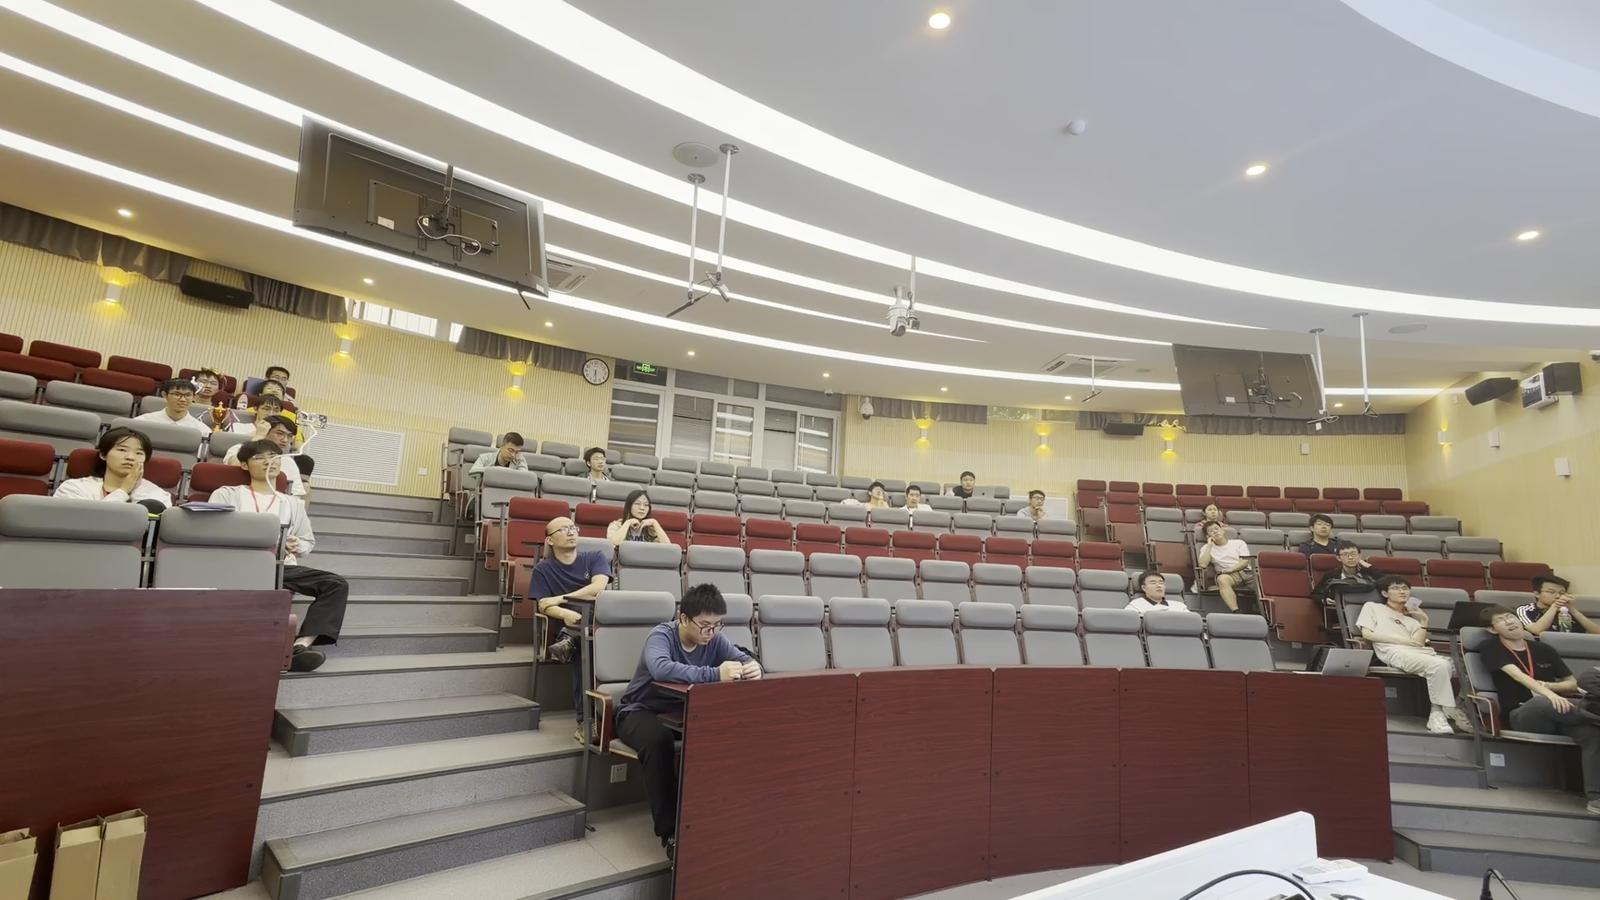
\includegraphics[width=\linewidth]{taitou/original_frame.png}
        \caption{原始课堂帧}
    \end{subfigure}
    \hfill
    \begin{subfigure}{0.48\textwidth}
        \centering
        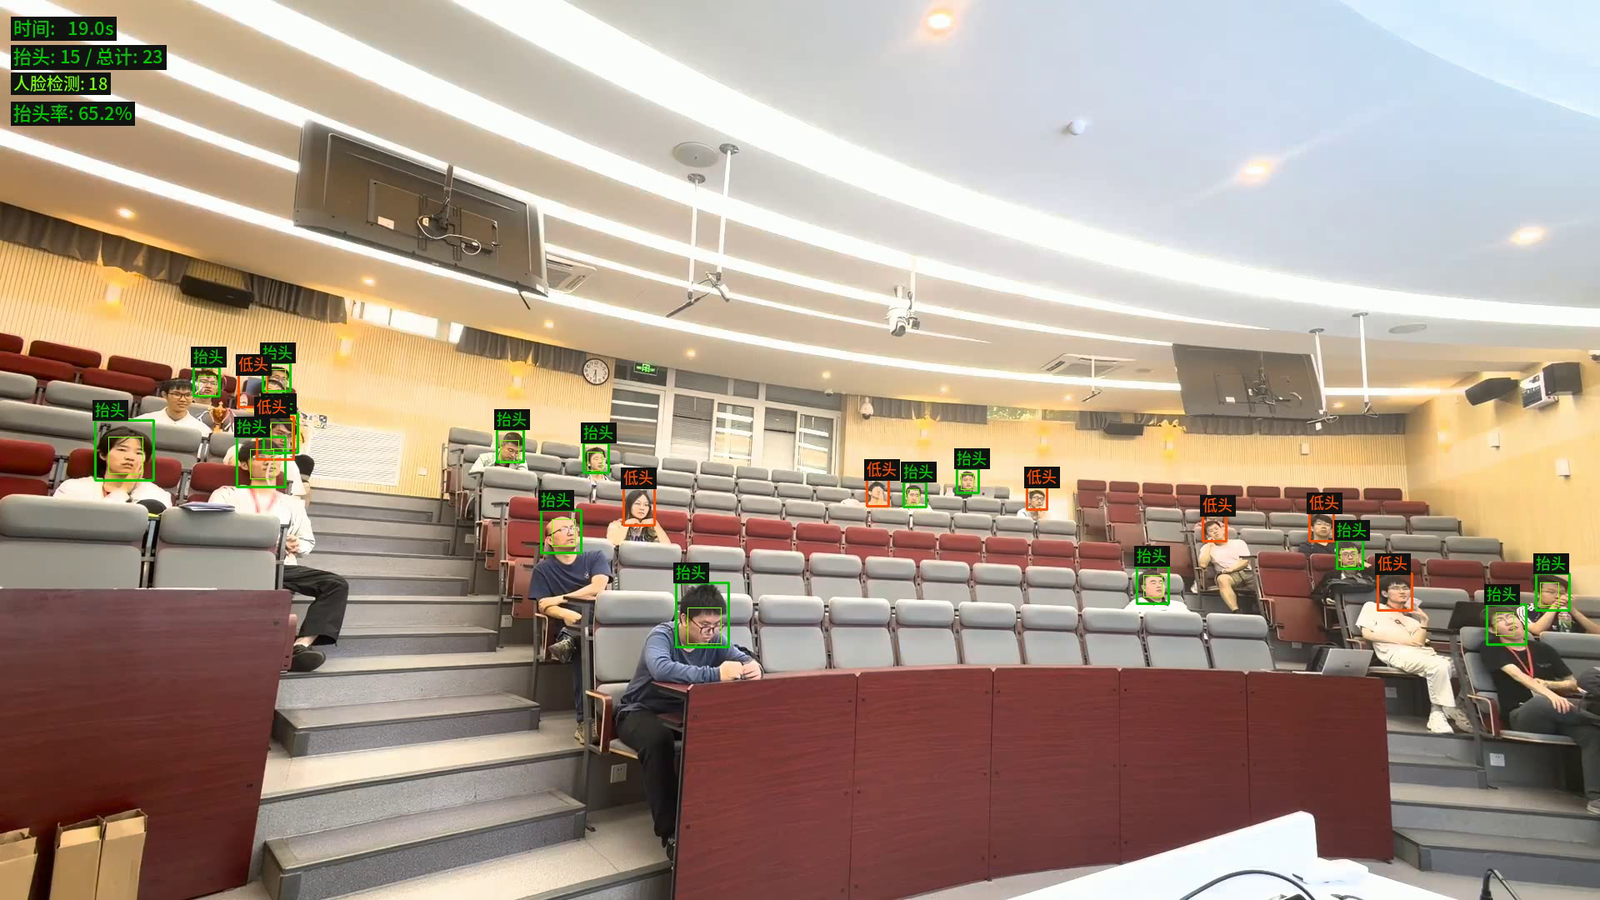
\includegraphics[width=\linewidth]{taitou/detect_overlay.png}
        \caption{检测结果叠加}
    \end{subfigure}
    \caption{前置摄像机学生区域检测结果}
    \label{fig:taitou_original_overlay}
\end{figure}

检测叠加图中，绿色框表示抬头，橙色框表示低头，两类框来自头部状态 YOLO 模型。左上角同步显示时间、抬头人数、学生总数、人脸数量和抬头率，其中人脸数量来自人脸 YOLO 模型。检测框和统计值保持对应，便于检查单帧结果。

状态判定以头部区域外观为依据。正向头部通常判为抬头，俯向桌面的头部判为低头。人脸模型只提供可见人脸数量，用于观察正脸可见程度，最终抬头率仍按头部状态模型计算。

\begin{figure}[H]
    \centering
    \begin{subfigure}{0.32\textwidth}
        \centering
        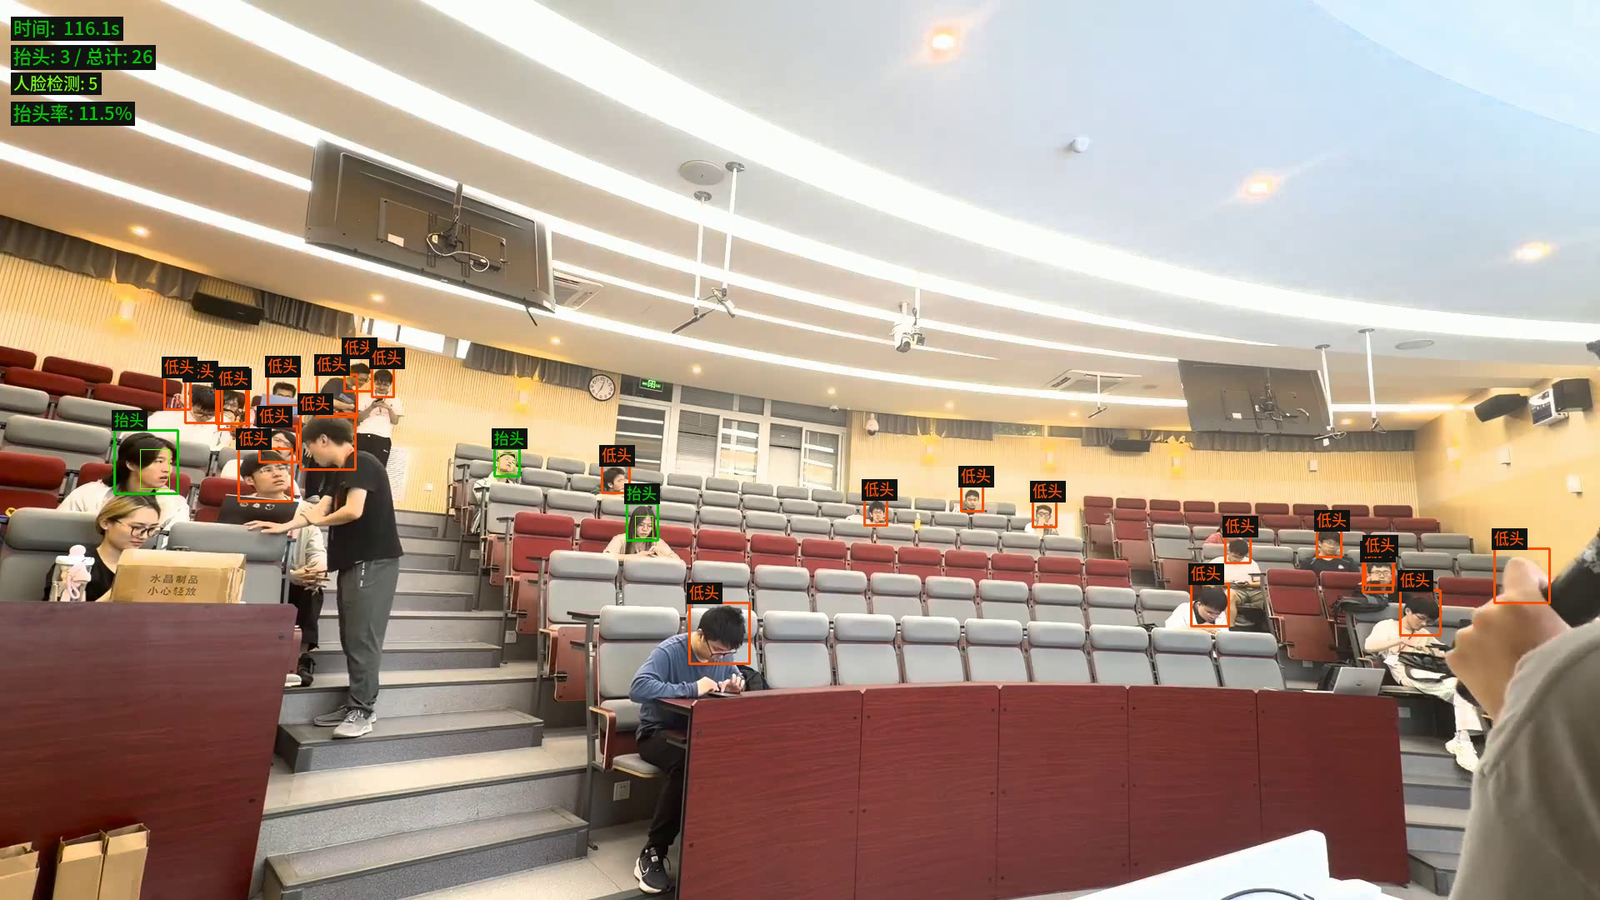
\includegraphics[width=\linewidth]{taitou/head_up_low.png}
        \caption{低抬头率片段}
    \end{subfigure}
    \hfill
    \begin{subfigure}{0.32\textwidth}
        \centering
        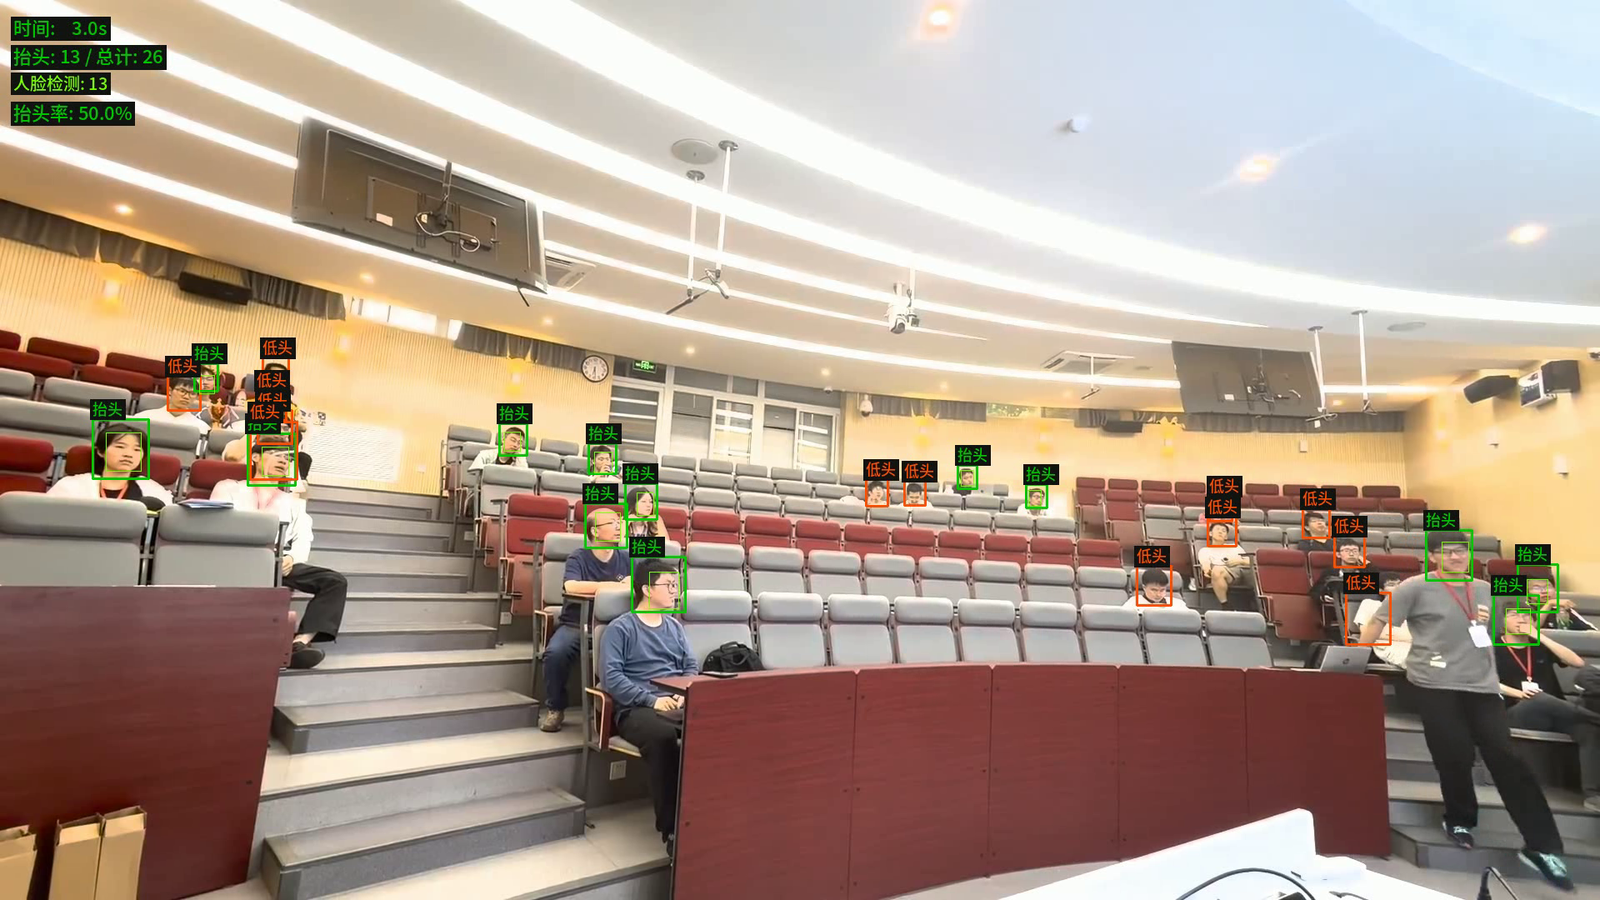
\includegraphics[width=\linewidth]{taitou/head_up_mid.png}
        \caption{中等抬头率片段}
    \end{subfigure}
    \hfill
    \begin{subfigure}{0.32\textwidth}
        \centering
        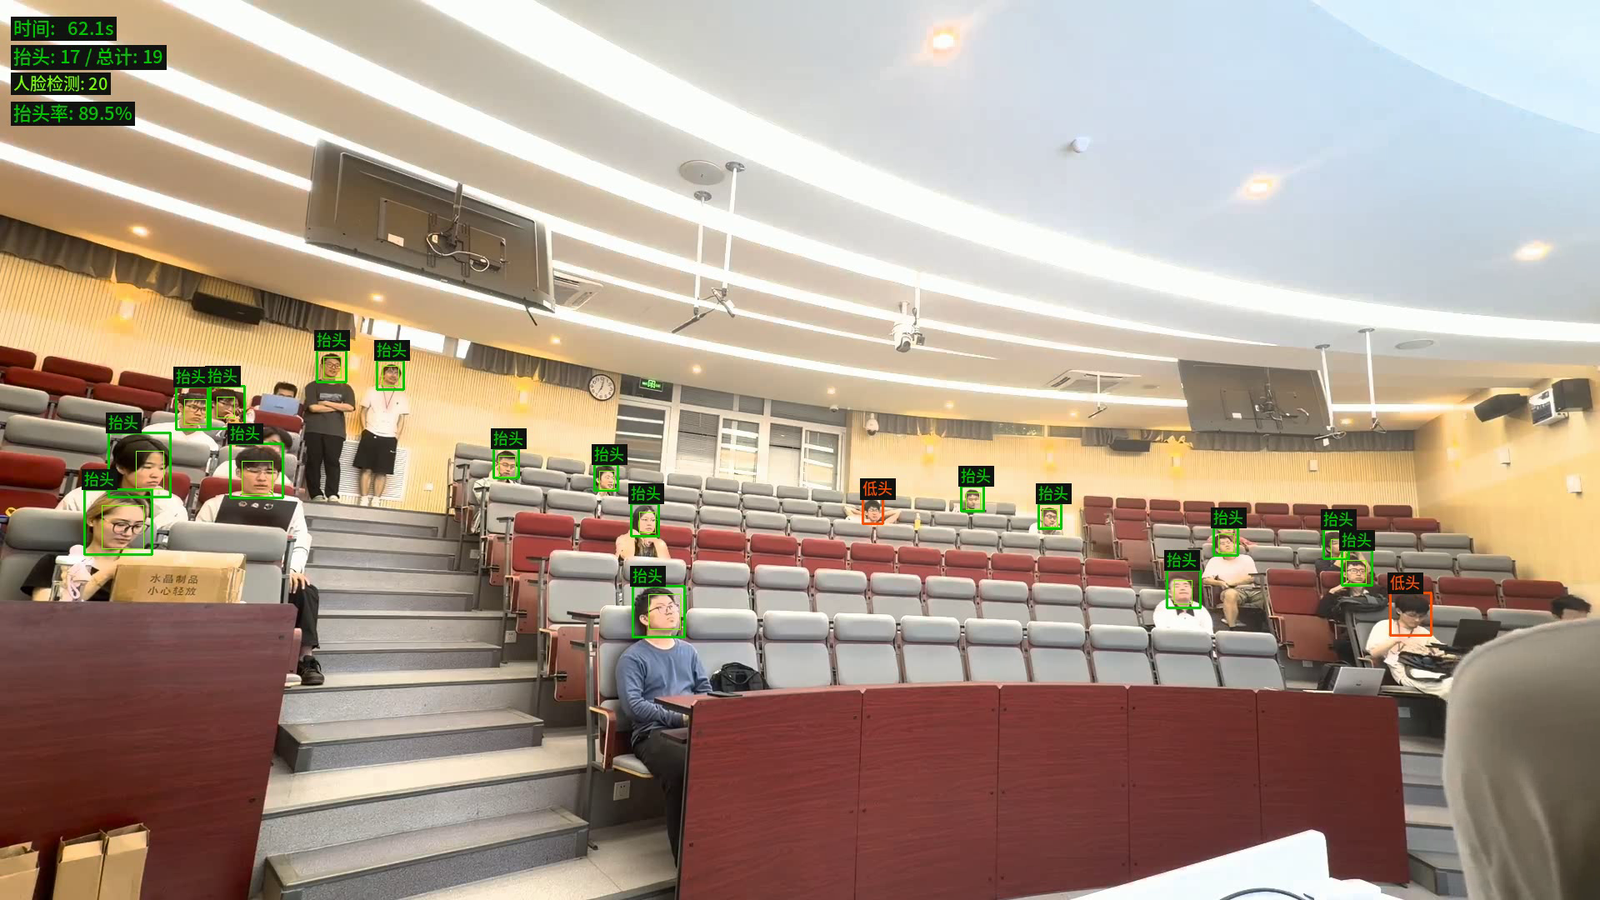
\includegraphics[width=\linewidth]{taitou/head_up_high.png}
        \caption{高抬头率片段}
    \end{subfigure}
    \caption{不同抬头率水平下的检测结果}
    \label{fig:taitou_levels}
\end{figure}

图 \ref{fig:taitou_levels} 展示低、中、高三种抬头率片段。低抬头率片段中低头目标占比较高，抬头率为 $11.5\%$；中等片段中两类目标数量接近，抬头率为 $50.0\%$；高抬头率片段中大部分学生被判为抬头，抬头率为 $89.5\%$。三组截图显示抬头率随群体头部姿态变化同步变化。

课堂画面存在遮挡和远距离小目标，单帧结果会有波动。实验用滑动窗口平滑抬头率，保留整体变化趋势。

\begin{figure}[H]
    \centering
    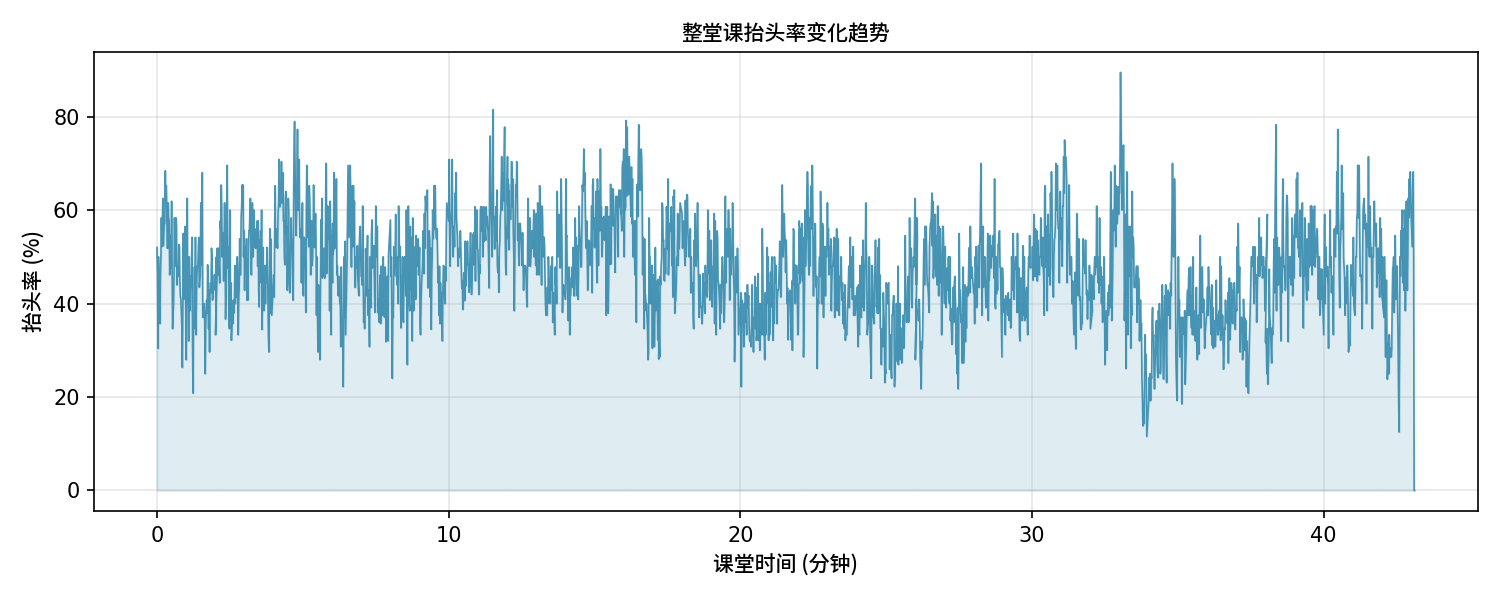
\includegraphics[width=0.95\textwidth]{taitou/rate_trend.png}
    \caption{整堂课抬头率变化趋势}
    \label{fig:taitou_trend}
\end{figure}

图 \ref{fig:taitou_trend} 展示整堂课抬头率趋势。曲线整体处于中等区间，局部有上升和下降。上升段表示更多学生面向前方，下降段表示低头比例增加。趋势曲线反映群体状态，比单帧结果更稳定。

实验结果说明，抬头率模块可以完成单帧检测、逐帧统计和整堂课趋势输出。叠加图用于检查检测结果，低中高截图用于展示不同状态，趋势图用于观察课堂过程中的连续变化。



\subsection{系统综合分析}

系统综合分析只基于抬头率序列展开。每个采样点包含时间戳、抬头人数、低头人数、学生总数和抬头率。系统先检查单帧叠加结果，再查看低中高片段，最后读取整堂课趋势曲线。三类结果对应局部检测、状态对比和整体走势。

从趋势上看，抬头率并非稳定常数，而是随课堂过程持续波动。高抬头率区间说明更多学生面向前方，低抬头率区间说明低头姿态增多。该指标不直接判断学习效果，只记录视觉姿态比例。抬头率适合作为课堂状态分析的基础数据，后续可再与课件、语音和互动信息结合。


\section{总结与展望}

\subsection{完成情况与成果}

\subsection{存在问题}


\subsection{成员分工}

小组分工按照课件识别、学生行为分析和系统融合三个方向展开，各成员在完成负责模块的同时共同参与数据采集、实验测试和报告整理。

\begin{itemize}
    \item \textbf{王思潮}：负责学生检测和人脸检测数据整理，完成 YOLO 模型训练、参数优化和抬头状态判定模块实现。
    \item \textbf{姚述军}：负责OCR 文字识别和页面切换检测模块，实现课件时间轴生成、实验统计和系统联调。
    \item \textbf{谢秋凡}：负责双摄像机视频采集、数据标注和时间轴对齐逻辑，实现课件区域提取、透视变换。
\end{itemize}


\begin{thebibliography}{99}
\bibitem{yang2019classroom} Yang Y, Zhan Y, Guo M, et al. In-classroom learning analytics based on student behavior, topic and teaching characteristic mining. Proceedings of the IEEE International Conference on Advanced Learning Technologies, 2019.

\bibitem{classmind2025} Chen L, Zhao Y, Li S, et al. ClassMind: Scaling Classroom Observation and Instructional Feedback with Multimodal AI. arXiv preprint arXiv:2503.11018, 2025.

\bibitem{fan2023yolov7} Fan Y, Wang Z, Liu Q, et al. Student Classroom Behavior Detection based on YOLOv7-BRA and Multi-Model Fusion. Proceedings of the IEEE Conference on Computer Vision and Pattern Recognition Workshops, 2023.

\bibitem{gao2026} Gao X, Hang J. ALC-YOLOv8s: Attention-based Lightweight Convolution for Dense Student Detection in Classroom. arXiv preprint arXiv:2601.07321, 2026.

\bibitem{acm2018attention} Huang Y, Chen K, Wang J. Estimation of Student Classroom Attention Using Head Motion Coherence. Proceedings of the ACM International Conference on Multimedia, 2018.

\bibitem{daisee2018} Chhokra J, Bhattacharya U, Paria B, et al. DAiSEE: A Dataset for Affect and Engagement Recognition in Classroom Environment. Proceedings of the ACM International Conference on Multimodal Interaction, 2018.

\bibitem{nougat2023} Blecher L, Chiu G C, Keung J, et al. Nougat: Neural Optical Understanding for Academic Documents. arXiv preprint arXiv:2308.13428, 2023.

\bibitem{layoutlm2020} Xu Y, Li M, Cui L, et al. LayoutLM: Pre-training of Text and Layout Document for Key Information Extraction. arXiv preprint arXiv:1912.13318, 2020.

\bibitem{nscr2026} Wang Z, Liu H, Chen Q, et al. Reliable Classroom AI via Neuro-Symbolic Multimodal Reasoning. arXiv preprint arXiv:2602.08456, 2026.

\bibitem{aamla2026} Zhang Y, Kim J, Park S, et al. AAMLA: Affinity-Aligned Multimodal Learning Analytics. arXiv preprint arXiv:2601.09274, 2026.

\bibitem{llmattention2026} Li R, Wang S, Chen K, et al. Can LLMs Reason About Attention? Towards Zero-Shot Analysis of Multimodal Classroom Behavior. arXiv preprint arXiv:2604.10234, 2026.

\bibitem{openface2020} Baltrusaitis T, Zadeh A, Lim Y C, et al. OpenFace 2.0: Facial Behavior Analysis Toolkit. Proceedings of the IEEE International Conference on Automatic Face and Gesture Recognition, 2020.

\bibitem{mediapipe2020} Lugaresi C, Tang J, Nash H, et al. MediaPipe: A Framework for Building Perception Pipelines. arXiv preprint arXiv:1906.08172, 2020.

\bibitem{yolov7} Wang C Y, Bochkovskiy A, Liao H Y M. YOLOv7: Trainable bag-of-freebies sets new state-of-the-art for real-time object detectors. Proceedings of the IEEE Conference on Computer Vision and Pattern Recognition, 2023.

\bibitem{redmon2016yolo} Redmon J, Divvala S, Girshick R, Farhadi A. You Only Look Once: Unified, Real-Time Object Detection. Proceedings of the IEEE Conference on Computer Vision and Pattern Recognition, 2016.

\bibitem{bochkovskiy2020yolov4} Bochkovskiy A, Wang C Y, Liao H Y M. YOLOv4: Optimal Speed and Accuracy of Object Detection. arXiv preprint arXiv:2004.10934, 2020.

\bibitem{jocher2023ultralytics} Jocher G, Chaurasia A, Qiu J. Ultralytics YOLO. 2023.

\bibitem{liao2020real} Liao M, Wan Z, Yao C, Chen K, Bai X. Real-Time Scene Text Detection with Differentiable Binarization. Proceedings of the AAAI Conference on Artificial Intelligence, 2020.

\bibitem{shi2016crnn} Shi B, Bai X, Yao C. An End-to-End Trainable Neural Network for Image-Based Sequence Recognition and Its Application to Scene Text Recognition. IEEE Transactions on Pattern Analysis and Machine Intelligence, 2016.

\bibitem{du2020ppocr} Du Y, Li C, Guo R, Yin X, Liu W, Zhou J, Bai Y, Yu Z, Yang Y, Dang Q, Wang H. PP-OCR: A Practical Ultra Lightweight OCR System. arXiv preprint arXiv:2009.09941, 2020.

\bibitem{bradski2000opencv} Bradski G. The OpenCV Library. Dr. Dobb's Journal of Software Tools, 2000.

\bibitem{bytetrack2022} Zhang Y, Wang P, Chai X, et al. ByteTrack: Multi-Object Tracking by Associating Every Detection Box. Proceedings of the European Conference on Computer Vision, 2022.

\bibitem{dtw2006} Berndt D J, Clifford J. Finding patterns in time series. Advances in Knowledge Discovery and Data Mining, 2006: 229-248.

\bibitem{donut2022} Kim G, Son S, Kim J. Donut: Document Understanding Transformer. arXiv preprint arXiv:2212.02728, 2022.

\bibitem{retinaface2019} Deng J, Guo J, Ververas E, et al. RetinaFace: Single-Shot Multi-Level Face Localisation in the Wild. Proceedings of the IEEE Conference on Computer Vision and Pattern Recognition, 2020.

\bibitem{6drepnet2022} Kumar A, GV R, et al. 6DRepNet: 6D Rotation Representation for Efficient Head Pose Estimation. arXiv preprint arXiv:2204.00640, 2022.

\bibitem{gcnengagement2019} Li D, Opie L, et al. Enhancing Student Engagement Recognition through Attention Mechanism and Graph Convolutional Network. arXiv preprint arXiv:1909.04486, 2019.
\end{thebibliography}

\end{document}